\section{Models}
Các đối tượng này được đọc từ file .obj và có vật liệu tương ứng đọc từ file .mtl. Ở đây chúng em sử dụng phần mềm Blneder để vẽ các đối tượng rồi xuất ra file .obj ứng với dữ liệu mô hình và file .mtl ứng với vật liệu của đối tượng.

\subsection{Ngôi nhà}
\begin{center}
    \begin{figure}[!h]
        \centering
        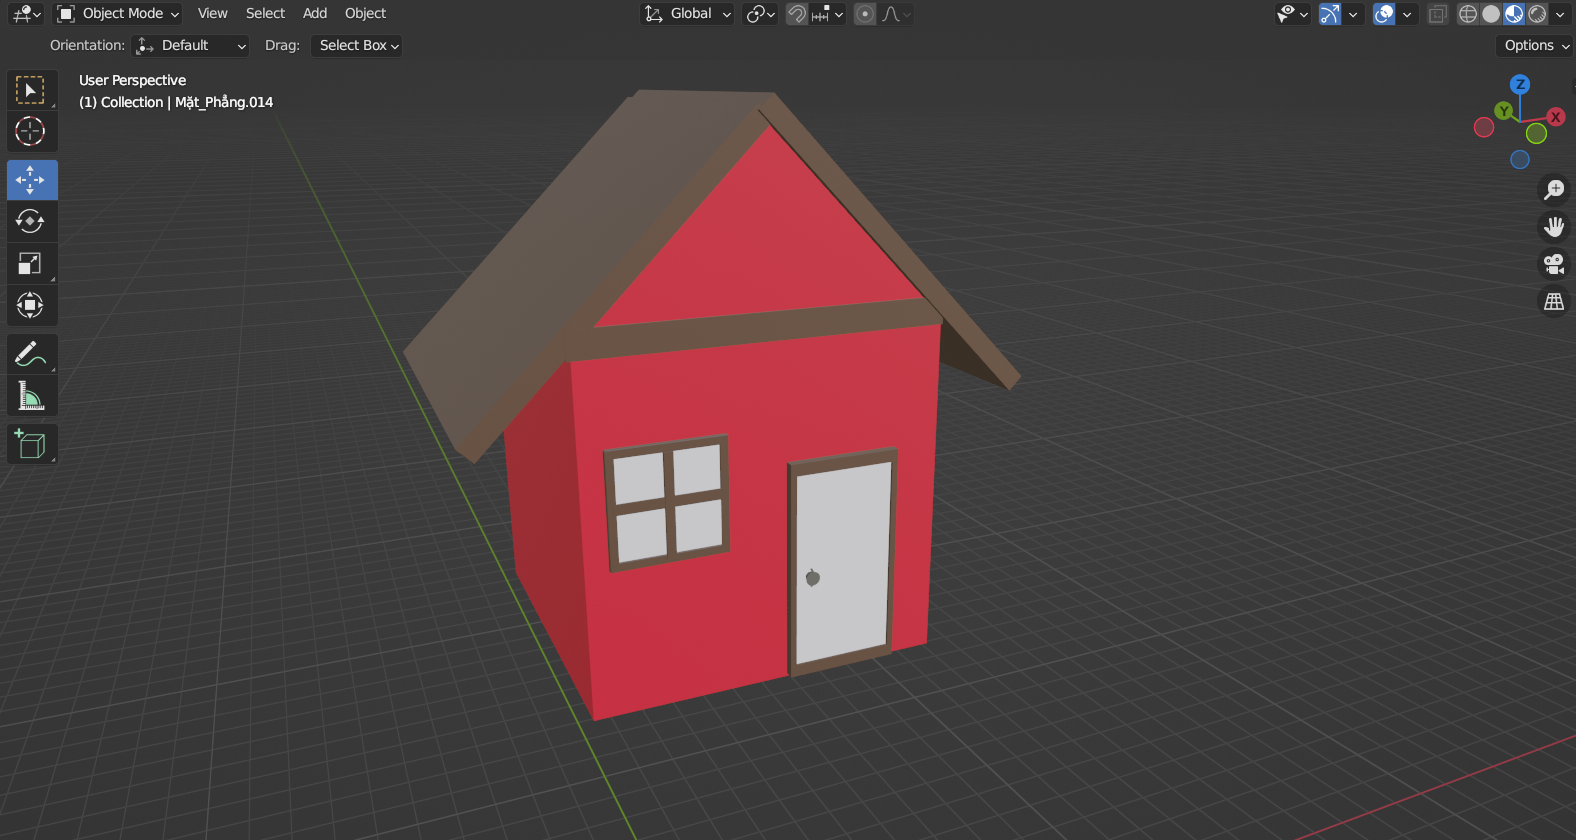
\includegraphics[scale = 0.4]{contents/house.png}
        \caption{Model bên ngoài ngôi nhà dựng bằng Blender}
    \end{figure}
\end{center}
\subsection{Chi tiết bên trong ngôi nhà}
\begin{center}
    \begin{figure}[!h]
        \centering
        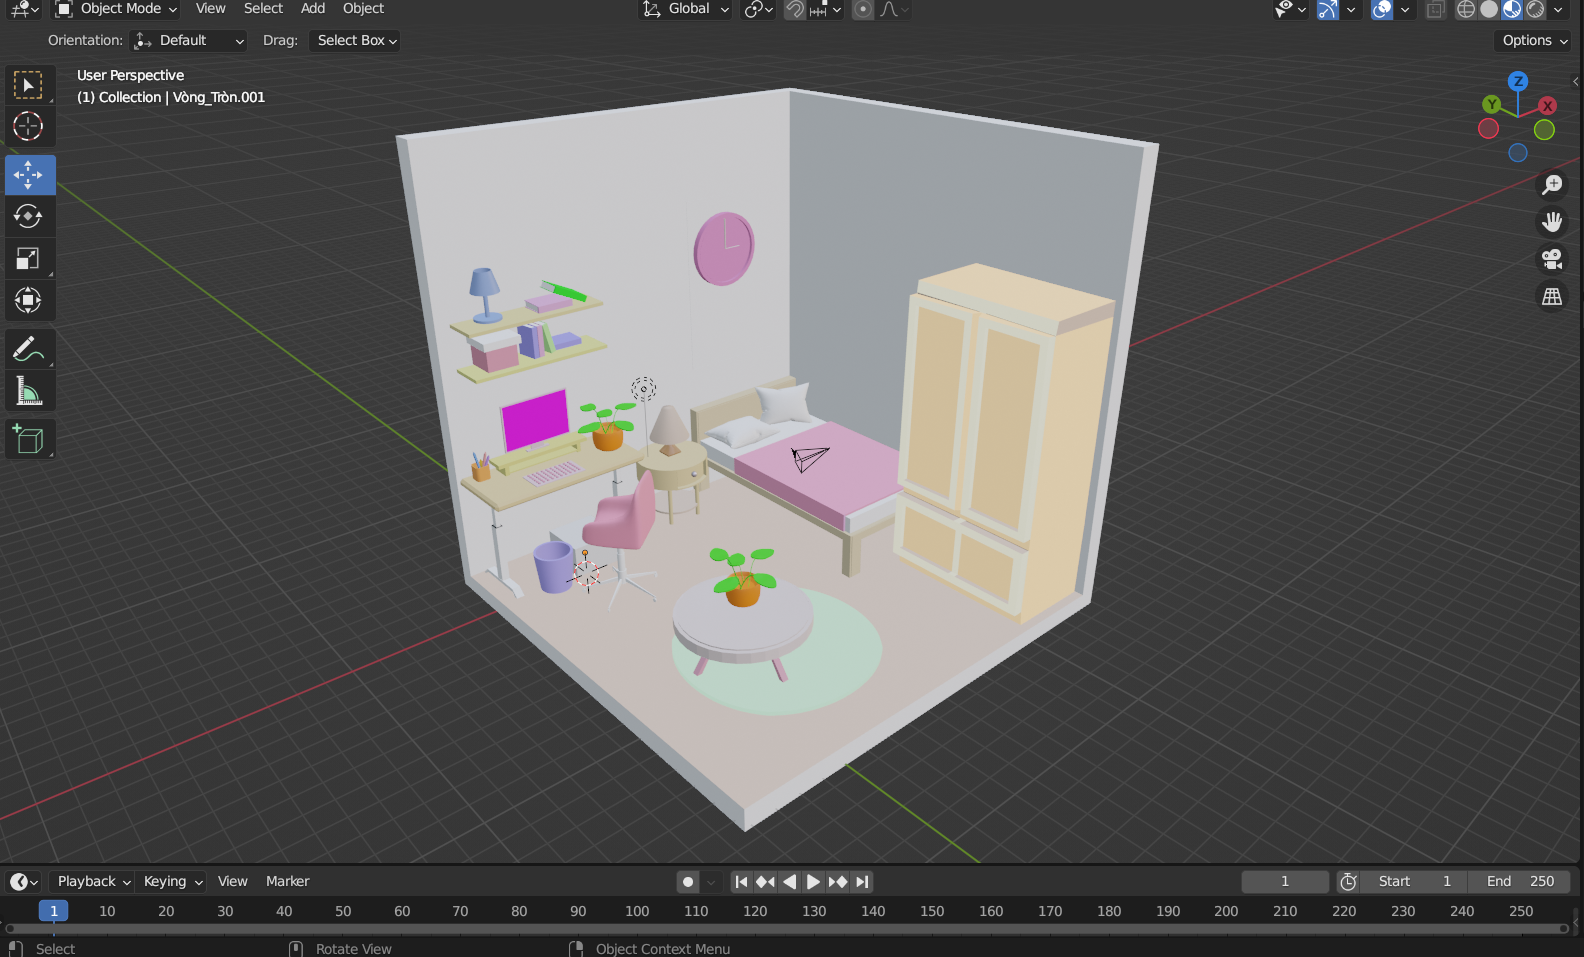
\includegraphics[scale = 0.35]{contents/fullhouse.png}
        \caption{Model chi tiết trong nhà dựng bằng Blender}
    \end{figure}
\end{center}

\newpage
\subsection{Cây}
\begin{center}
    \begin{figure}[!h]
        \centering
        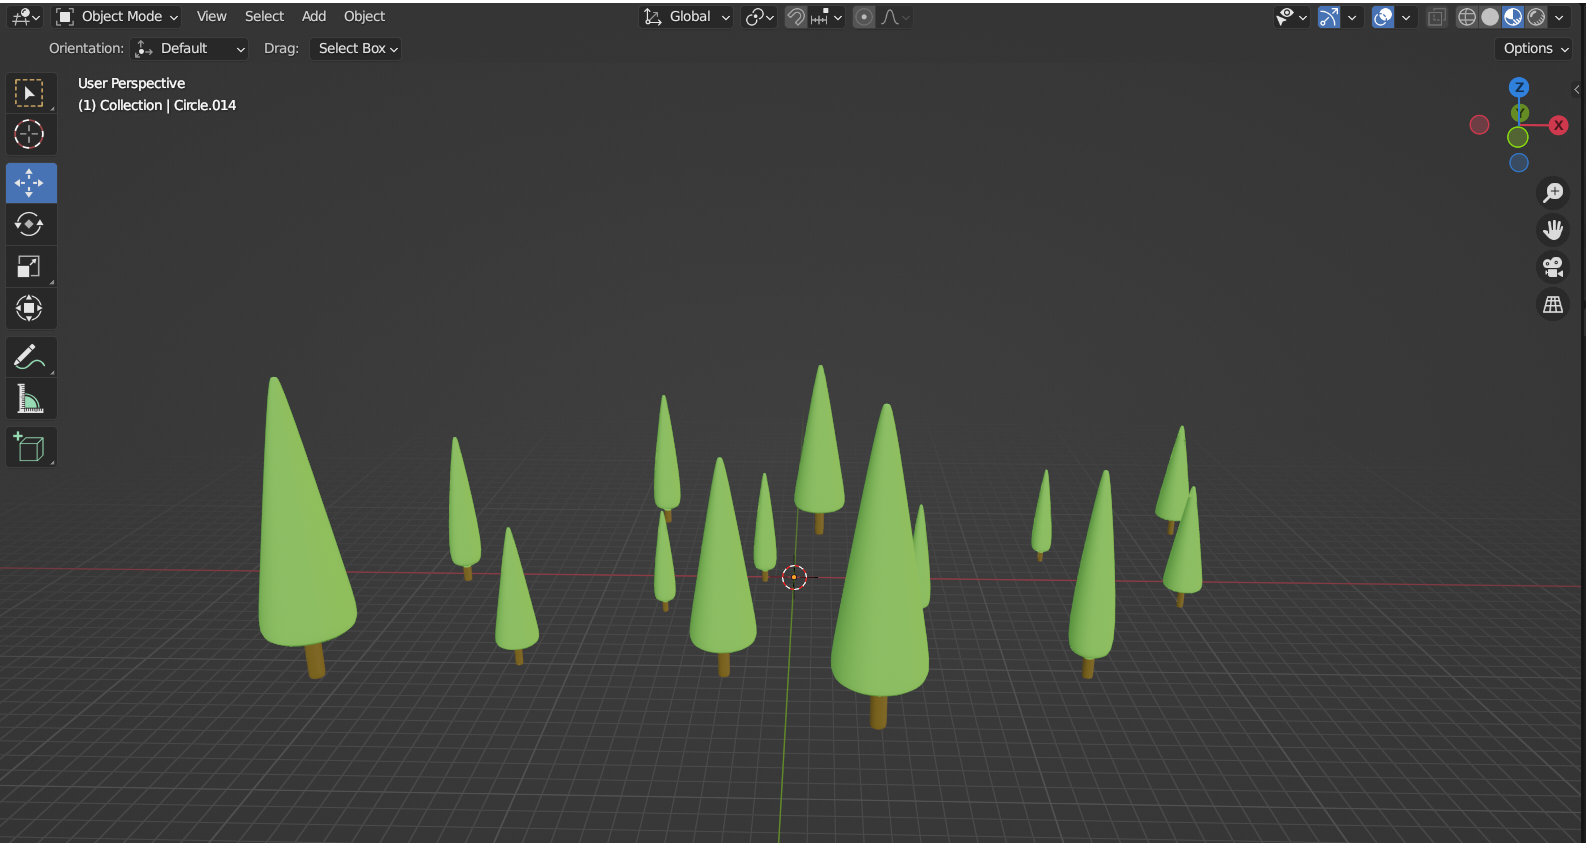
\includegraphics[scale = 0.35]{contents/tree.png}
        \caption{Model rừng cây dựng bằng Blender}
    \end{figure}
\end{center}


\subsection{Mây}
\begin{center}
    \begin{figure}[!h]
        \centering
        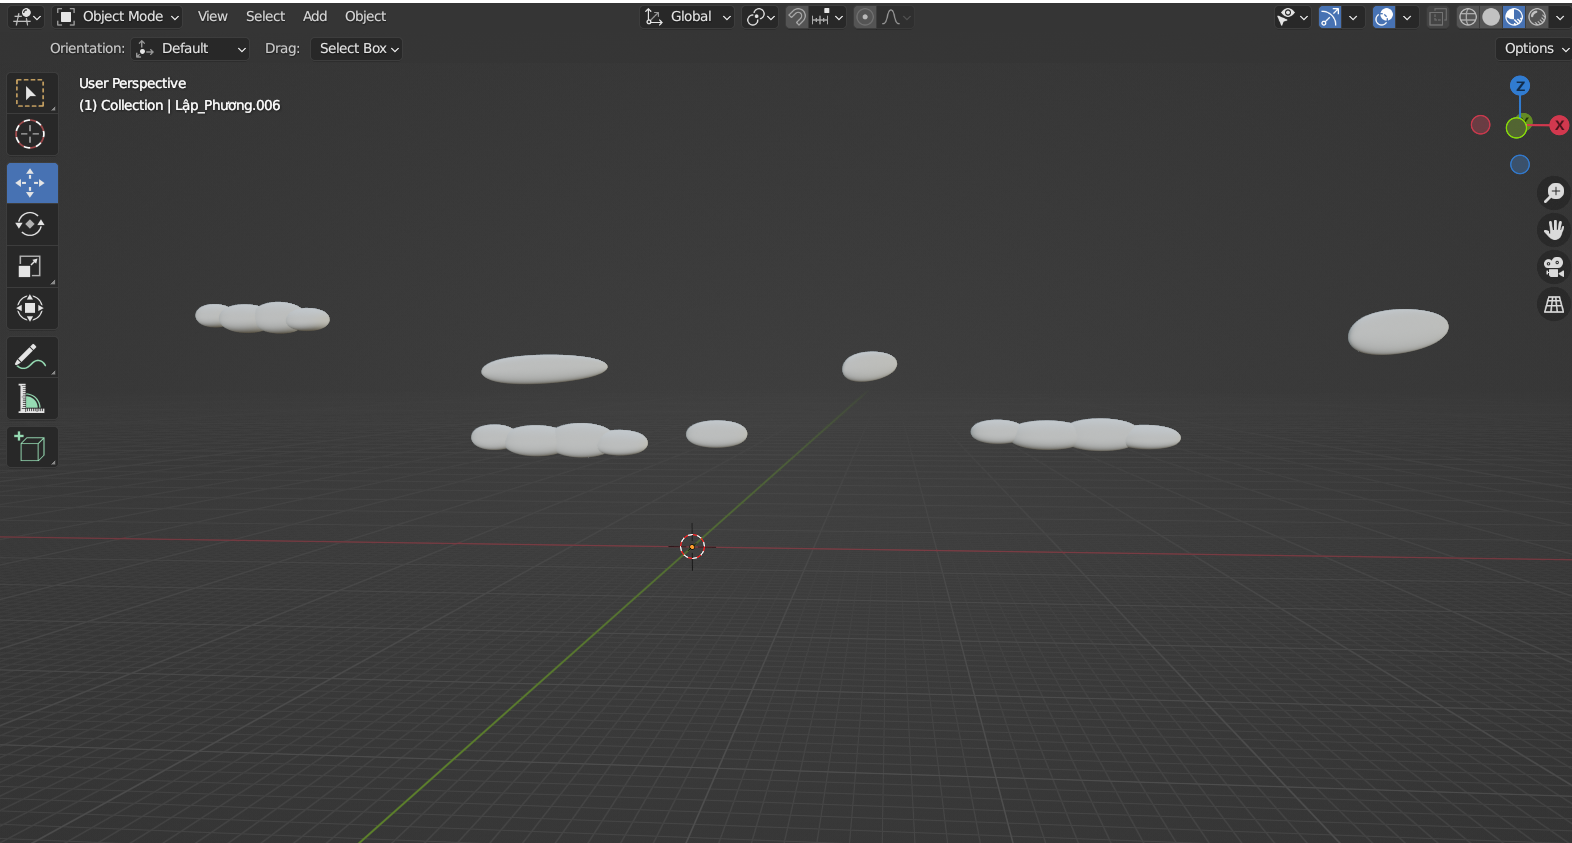
\includegraphics[scale = 0.35]{contents/cloud.png}
        \caption{Model các đám mây dựng bằng Blender}
    \end{figure}
\end{center}